\documentclass[conference,10pt]{IEEEtran}
% Re-allow e.g. the \thanks command.
\IEEEoverridecommandlockouts

\usepackage[dvipsnames]{xcolor}
% to be able to draw some self-contained figs
\usepackage{tikz}
\usepackage{amsmath}
\usepackage{minted}
% \usepackage[utf8]{inputenc}
\usepackage{csquotes}
\usepackage{amsthm}
\usepackage{siunitx}
\usepackage[caption=false]{subfig}
\usepackage{listings}

%%%% listings pkg: %%%%

% \lstloadlanguages{Haskell}

\lstset{
  basicstyle=\scriptsize\ttfamily,
  %mathescape=true,
  %numbers=left,
  mathescape=false,
  aboveskip=\medskipamount,
  belowskip=\smallskipamount,
  showspaces=false,
  keywordstyle=,
  numberstyle=\tiny,
  numbersep=0pt,
  %stepnumber=2,
  tabsize=2,
  %extendedchars=true,
  breaklines=false,
  %keywordstyle=\color{black}
  }
  % TODO this inherited or not from other lstnewenvironment
\newcommand{\lstcd}[1]{\lstinline[basicstyle=\ttfamily\footnotesize]{#1}}

% this style is used for long/verbatim notes (not text) in the paper
\lstdefinestyle{meta}
  {basicstyle=\scriptsize\ttfamily\color{magenta}}

\lstnewenvironment{myc}
    {\lstset{}%
      \csname lst@SetFirstLabel\endcsname}
    {\csname lst@SaveFirstLabel\endcsname}
    \lstset{
      basicstyle=\scriptsize\ttfamily,
      mathescape=false,
      language=C,
      lineskip=1pt,
      showspaces=false,
      keywordstyle=,
      flexiblecolumns=false,
      basewidth={0.5em,0.45em}
    }

\lstnewenvironment{code}
    {\lstset{}%
      \csname lst@SetFirstLabel\endcsname}
    {\csname lst@SaveFirstLabel\endcsname}
    \lstset{
      mathescape=false,
      language=Haskell,
      lineskip=1pt,
      showspaces=false,
      numbersep=0pt,
      keywordstyle=,
      basicstyle=\scriptsize\ttfamily,
      flexiblecolumns=false,
      basewidth={0.5em,0.45em},
      literate={+}{{$+$}}1 {/}{{$/$}}1 {*}{{$*$}}1 {=}{{$=$}}1
               {>}{{$>$}}1 {<}{{$<$}}1 {\\}{{$\lambda$}}1
               {\\\\}{{\char`\\\char`\\}}1
               {->}{{$\rightarrow$}}2 {>=}{{$\geq$}}2 {<-}{{$\leftarrow$}}2
               {<=}{{$\leq$}}2 {=>}{{$\Rightarrow$}}2 
          %     {\ .\ }{{$\circ$}}2
               {>>}{{>>}}2 {>>=}{{>>=}}2
               {|}{{$\mid$}}1               
    }
    % literate haskell assumes \begin{code}

% when we don't want Haskell to execute the code in paper:
% Alts    
%   \newenvironment{codeNoExecute}{\code}{\endcode} 
%   \let\codeNoExecute\code
%   \let\endcodeNoExecute\endcode
%   the below, just duplicated from above:
\lstnewenvironment{codeNoExecute}
    {\lstset{}%
      \csname lst@SetFirstLabel\endcsname}
    {\csname lst@SaveFirstLabel\endcsname}
    \lstset{
      mathescape=false,
      language=Haskell,
      lineskip=1pt,
      showspaces=false,
      keywordstyle=,
      basicstyle=\scriptsize\ttfamily,
      flexiblecolumns=false,
      basewidth={0.5em,0.45em},
      literate={+}{{$+$}}1 {/}{{$/$}}1 {*}{{$*$}}1 {=}{{$=$}}1
               {>}{{$>$}}1 {<}{{$<$}}1 {\\}{{$\lambda$}}1
               {\\\\}{{\char`\\\char`\\}}1
               {->}{{$\rightarrow$}}2 {>=}{{$\geq$}}2 {<-}{{$\leftarrow$}}2
               {<=}{{$\leq$}}2 {=>}{{$\Rightarrow$}}2 
           %   {\ .\ }{{$\circ$}}2
               {>>}{{>>}}2 {>>=}{{>>=}}2
               {|}{{$\mid$}}1               
    }
    % literate haskell assumes \begin{code}

    
\usepackage{hyperref}
\usepackage[capitalise]{cleveref}
  % i.e., you use '\cref{x}' rather than "Figure \ref{x}"
% inlined bib file
\usepackage{filecontents}

% SYSTEM OF ANNOTATIONS:

\newcommand{\pwnote}[1]{\textcolor{blue}{[PW: #1]}}
\newcommand{\mtnote}[1]{\textcolor{BlueGreen}{[MT: #1]}}
\newcommand{\whnote}[1]{\textcolor{Cyan}{[WH: #1]}}
\newcommand{\wwnote}[1]{\textcolor{orange}{[WW: #1]}}

\newcommand{\pwtodo}[1]{\pwnote{TODO: #1}}
\newcommand{\mttodo}[1]{\mtnote{TODO: #1}}
\newcommand{\whtodo}[1]{\whnote{TODO: #1}}


\newcommand{\info}[1]{\textcolor{brown}{[[#1]]}}
\newcommand{\note}[1]{\noteYes{#1}}  
\newcommand{\noteNo}[1]{}  % way to remove all notes.
\newcommand{\noteYes}[1]{\textcolor{red}{[[#1]]}}
\newcommand{\todo}[1]{\note{TODO: #1}}
\newcommand{\todoa}[1]{\todo{[\#A]: #1}}
\newcommand{\todob}[1]{\todo{[\#B]: #1}}
\newcommand{\todoc}[1]{\todo{[\#C]: #1}}
\newcommand{\old}[1]{\textcolor{orange}{[[OLD: #1]]}}

\newcommand{\haskellnote}[1]{#1}
  % ever add formatting to? Just used to indicate notes to non-Haskellers
\newcommand{\keypoint}[1]{{\bf{#1}}}
  % TODO: boxed frame maybe?
\newcommand{\paragraphsection}[1]{\vspace{7pt}\noindent{\textit{#1}}}
  % use this for "Initial Results" or for sections at the lowest level.
  % TODO: is the formatting sufficiently smaller than level 2 sections?
 
\sisetup{group-separator={,}, group-minimum-digits=4}



\begin{document}

\date{}

% make title bold and 14 pt font (Latex default is non-bold, 16 pt)
\title{Strengthening Weak Links in the PDF Trust Chain}

\author{
    \IEEEauthorblockN{ William Harris, Mark Tullsen }%
    \IEEEauthorblockA{\small Galois, Inc.\\
    \texttt{\{wrharris, tullsen\}@galois.com}} \and
    \IEEEauthorblockN{Peter Wyatt}
    \IEEEauthorblockA{\small PDF Association\\
    \texttt{peter.wyatt@pdf.org}}
}

\maketitle

% abstract:
\begin{abstract}
  % context:
  Conventional data-description languages, such as context-free
  grammars, naturally define formats in which the semantic
  interpretation of a large segment of input depends hierarchically on
  the semantic interpretations of its sub-segments.
  %
  They cannot be applied to many practical and security-critical
  formats---including the Portable Document Format (PDF)---in which
  the interpretation of a segment as a \emph{Document Object Model
    (DOM)} graph depends on a concept of reference and complex
  contextual data that binds data objects to references
  \textcolor{blue}{shouldn't this be "references to data objects"?}.
  %
  Such referential context itself must often be defined
  discontinuously and compressed, to satisfy practical constraints on
  usability and performance.
  \textcolor{blue}{Sorry - I don't understand this previous sentence. How about "The integrity of these references and their context ensures that the DOM graph is established from a basis of trust."?}

  % result:
  This paper describes a case study of a critical instance of such a
  design, namely the construction of PDF \emph{cross-reference tables},
  in the presence of potentially multiple incremental updates and multiple dialects expressing these references.
  %
  Over the course of case study, we found that the full definition of
  cross-reference data in PDF contains several subtleties that could be
  mis-implemented by natural implementations, but which can
  nevertheless be formalized using parser combinators in a
  data-definition language with constructs for explicitly capturing
  and updating input streams.
  %
  Our definition has served as a foundation for implementing format
  security analyses that arise naturally while constructing DOM's,
  including the analysis of document \emph{cavities} that may store
  unexamined data used to construct file \emph{polyglots}.
  
  \todo{need to be consistent in terminology: PDF Trust Chain vs Chain of Trust. Also be good to use this phrase in the Abstract}
\end{abstract}


% \section{[Meta-Notes for Authors]}

\begin{lstlisting}[style=meta]
CONVENTION:
 - using this lstlisting[style=meta] environment to capture
   text in outline form that has not been fleshed out / turned into prose.
\end{lstlisting}

\begin{lstlisting}[style=meta]
META NOTES:  
- aim for 12 pages (in 10pt)

TERMS (to actually use, and define when needed):
- ``complies with standard'', ``compatible with standard''
- Pre-DOM
- XRef (capitalized thus)
- Trust Chain (no quotes) [remove upper case?]
\end{lstlisting}

% content:
% ------------------------------------------------------------------------------
\section{Introduction}
\label{sec:intro}
% background: conventional grammars:
The task of parsing may be viewed as receiving a document in an
unstructured, serialized form, and trustably building its structured
representation.
%
For formats defined in conventional data-description languages that
correspond closely to well-understood classes of the Chomsky hierarchy
(i.e., context-free grammars, with regular expressions as a critical
special case), arguments of trustworthiness fall out naturally from
the definition of the format itself.
%
This is in part due to the fact that in such formats, the structured
representation of a large segment of a message is defined purely in
terms of the structure of its segments.

% real formats have DOMs, which involve names and references
However, these key properties concerning context-freedom critically do
not hold for many practical formats, which define a \emph{Document
  Object Model} (DOM): i.e., the result of parsing a document is a
graph between objects, each of which may contain values bound to a
large set of fields.
%
In such formats, it is infeasible to provide context-free definitions
of well-formedness because data objects that must satisfy critical
relations may not occur contiguously: related objects may not form a
tree-like hierarchy in the input stream.
%
Such formats typically introduce a notion of \emph{naming} or
\emph{reference} by which objects may refer to each other.
%
A critical practical example of this design pattern---and the
motivating example of our work---is the document object model of the
\emph{Portable Document Format (PDF)}~\cite{isotc171sc2wg8ISO32000220202020};
%
PDF data objects include an \emph{object identifier}, by which other
objects may refer to them.

% further complications: people want to do other fancy tricks with
% context tables
In such formats, the structures of references and context take on
central importance.
%
In practice, their structure is quite complex in order to support
practical demands.
%
E.g., PDF's \emph{cross-reference table} enables
% 
\textbf{(1)} the interpretation of documents to be strongly mutated by
appending content, via \emph{incremental updates};
%
\textbf{(2)} the reference structure to be compressed, via
standardized but non-trivial algorithms applied to
\emph{cross-reference streams}, potentially combined with conventional
cross-reference tables in \emph{hybrid reference files}; and
% 
\textbf{(3)} large documents to be partially processed incrementally,
using separated context, via \emph{linearization}.
%
The parsing of this reference and context information occurs before
DOM creation and DOM object validation, introducing a reliance on the
correctness of all \emph{pre-DOM} processing.

% security consequences:
Difficulties in expressing the structure and semantics of references
have resulted in critical security vulnerabilities.
%
The induced \emph{ambiguities} cause different parties
to assign wildly different semantic interpretations to the same
document.
%
Recently discovered attacks that compromise the integrity and
usability of digital
signatures~\cite{rohlmannBreakingSpecificationPDF2021,
  mainkaShadowAttacksHiding2021} use maliciously crafted
cross-reference tables. Our work has identified additional exploits
against digital signatures and PDF file integrity based on our
formalisms of PDF file structure and layout~\cite{cve25641}.

Furthermore, such formats invite document \emph{cavities}---segments
of a document that are not reflected in its semantic
interpretation---may store content that is completely unobservable to
parser clients.
%
Such cavities are a powerful mechanism for creating \emph{polyglot
  files} (i.e., files that unexpectedly belong to multiple formats),
which themselves have been used in recent critical system security
exploits~\cite{psychicPaper}.

% potential solutions and why they fail:
Context-free grammars and weaker formalisms are not suitable to define 
such formats in full detail.
%
In the conventional setting, a parser returns a semantic value that is
then potentially transformed by further computation, which itself be
defined in an attribute grammar or parser client logic.
%
The main limitation of such an approach is that computation on
semantic values must then itself effectively parse unstructured data
after computing partial contextual information;
%
such parsing logic is exactly what should be expressed declaratively
in a grammar and implemented by a generated parser.

% our solution: very careful parser combinators:
This paper explores a more powerful alternative: monadic parsers equipped 
with actions for explicitly capturing and setting the parser's input, run 
in a well-founded sequence of staged computations over semantic values.
%
This approach is explored within an industrial strength case study:
validating and parsing the reference tables that are needed to create 
an unambiguous and trustworthy PDF DOM.
%
However, our work is unique in that, to our knowledge, it constitutes
the first attempt to use such combinators to formalize a comprehensive
set of features and integrity relationships in PDF pre-DOM processing
that define referential context, specifically cross reference tables,
incremental updates, and cross reference table compression within
cross-reference streams.
These are the first stages in the PDF ``Trust Chain,'' and  strongly complements all
efforts that rely on a trustworthy formalization of reference in order
to validate properties of higher-level document abstraction defined in
terms of a DOM.

% background on parser combinators
In general, using parser combinators is not new: such combinators are
available widely available in the distributions of modern industrial
strength languages~\cite{leijen2001parsec,couprie2015nom,mundkurResearchReportParsley2020,bratus2017curing,willis2020staged}.
%
Moreover, with the recent interest in formalizing practical formats
and generating high-assurance parsers, such combinators have
specifically been applied to formalize components of the
PDF standard related to referential context.
%
PDF is a random-access binary file format
that must be processed from the most recent (latest) incremental
update through earlier edits back to the original document.
%
PDF cross-reference data defines byte offsets from the start of the
file to the start byte for each PDF object. PDF object identifiers may
also not be unique, as incremental updates may redefine existing
objects, or reinstate objects that were previously marked as free
(unused).
%
Thus, in order to correctly establish a final PDF DOM graph, it is
necessary to parse each appended incremental update in reverse
order.

% results
Our case study shows that such features can by formalized effectively.
%
The resulting definition is more subtle than what may be often be
implemented by inspecting the PDF standard or many extant documents:
in the process of producing our definition, we raised several issues
with the current PDF standard which have been acknowledged and
addressed by the PDF Association and the ISO.
%
However, there is nothing in the format definition that requires the
specific language of combinators to be employed: a key goal of our work is
to provide this formalized definition as a worked case study, to be
vetted and improved upon using definitions in other experimental data
definition languages as they are developed.

\paragraph*{Organization} The rest of this paper is organized as
follows:
%
\Cref{sec:pdf} explains the PDF format and discusses some of its
complexities and vulnerabilities;
%
\Cref{sec:parsing} discusses the details and surprising
complexities of actually \emph{parsing} the PDF format;
%
\Cref{sec:specifying} presents our specification of reference in detail;
%
\Cref{sec:implementation} discusses our implementation;
%
\Cref{sec:assessing} assesses our approach;
%
\Cref{sec:rel-work} reviews related work, and %
\Cref{sec:conclusion} concludes.


\section{The PDF Trust Chain \note{1.5pp}}
\label{sec:trust-chain}

\subsection{Trust Chains in General}
The term \emph{Trust Chain} (or ``Chain of Trust'') is used in multiple contexts, e.g.,
\emph{digital certificates}: a sequence of certificates signing certificates,
starting with a root certificate;
\emph{supply chain}: a product is no more reliable or secure than its
outsourced components;
\emph{trusted boot}: unless the bootloader is correct and non-malicious,
there can be no possibility of the operating system being the same;
\emph{software stacks}: upper layers are dependent upon lower layers (such as
system libraries) and vulnerabilities at the lower layers affect all higher layers.

The common idea is having layers
that rely on lower layers for their validity
(or components that rely on sub-components, etc.),
and the key lesson being:
{\bf{if a single layer of the trust chain 
  is flawed or suborned, then every layer relying on it
  is no longer capable of being trusted.}}

\mtnote{I used 'layer' in this subsection, but hereafter I'll be using
  'stage' (not phase/component/etc) for our concrete instance in PDF.}

\subsection{The Trust Chain of a PDF Parser}

% In \cref{sec:pdf-challenges}, we elaborated on the challenges of PDF.
% Parsing data-formats has a long history and many solutions ...
% Parsing formal languages also has a long history and many solutions ...
% PDF has aspects of both: this makes PDF challenging.
% But PDF ``parsing'' is not merely a matter of harder [difference of degree]
% but intrinsically more complex [a difference of kind!]:

\begin{figure}[t]
  \centering
  \begin{lstlisting}
    +-----------------------------------------------------+
    | 1. Find & parse header and trailer                  |<-- File
    +-----------------------------------------------------+
                       | offsets + ...
                       v
    +-----------------------------------------------------+
    | 2. Find & parse incremental updates                 |<-- File
    +-----------------------------------------------------+
                       | list of raw XRef maps
                       v
    +-----------------------------------------------------+
    | 3. Combine incremental updates                      |<-- File
    +-----------------------------------------------------+
                       | one XRef map
                       v
    +-----------------------------------------------------+
    | 4. Transform XRef map to object map (DOM)           |
    |    1. Parse uncompressed objects                 <--+-- File
    |    2. Decode streams & preprocess object streams <--+-- File
    |    3. Resolve type 2 object references           <--+-- File
    +-----------------------------------------------------+
                       | Object map (DOM)
                       v
    +-----------------------------------------------------+
    | 5. Validate candidate DOM                           |
    +-----------------------------------------------------+
                       | Object map (DOM)                                    
                       v
    +-----------------------------------------------------+
    | 6. Render DOM                                       |
    +-----------------------------------------------------+
                       | 
                       v
  \end{lstlisting}
  % 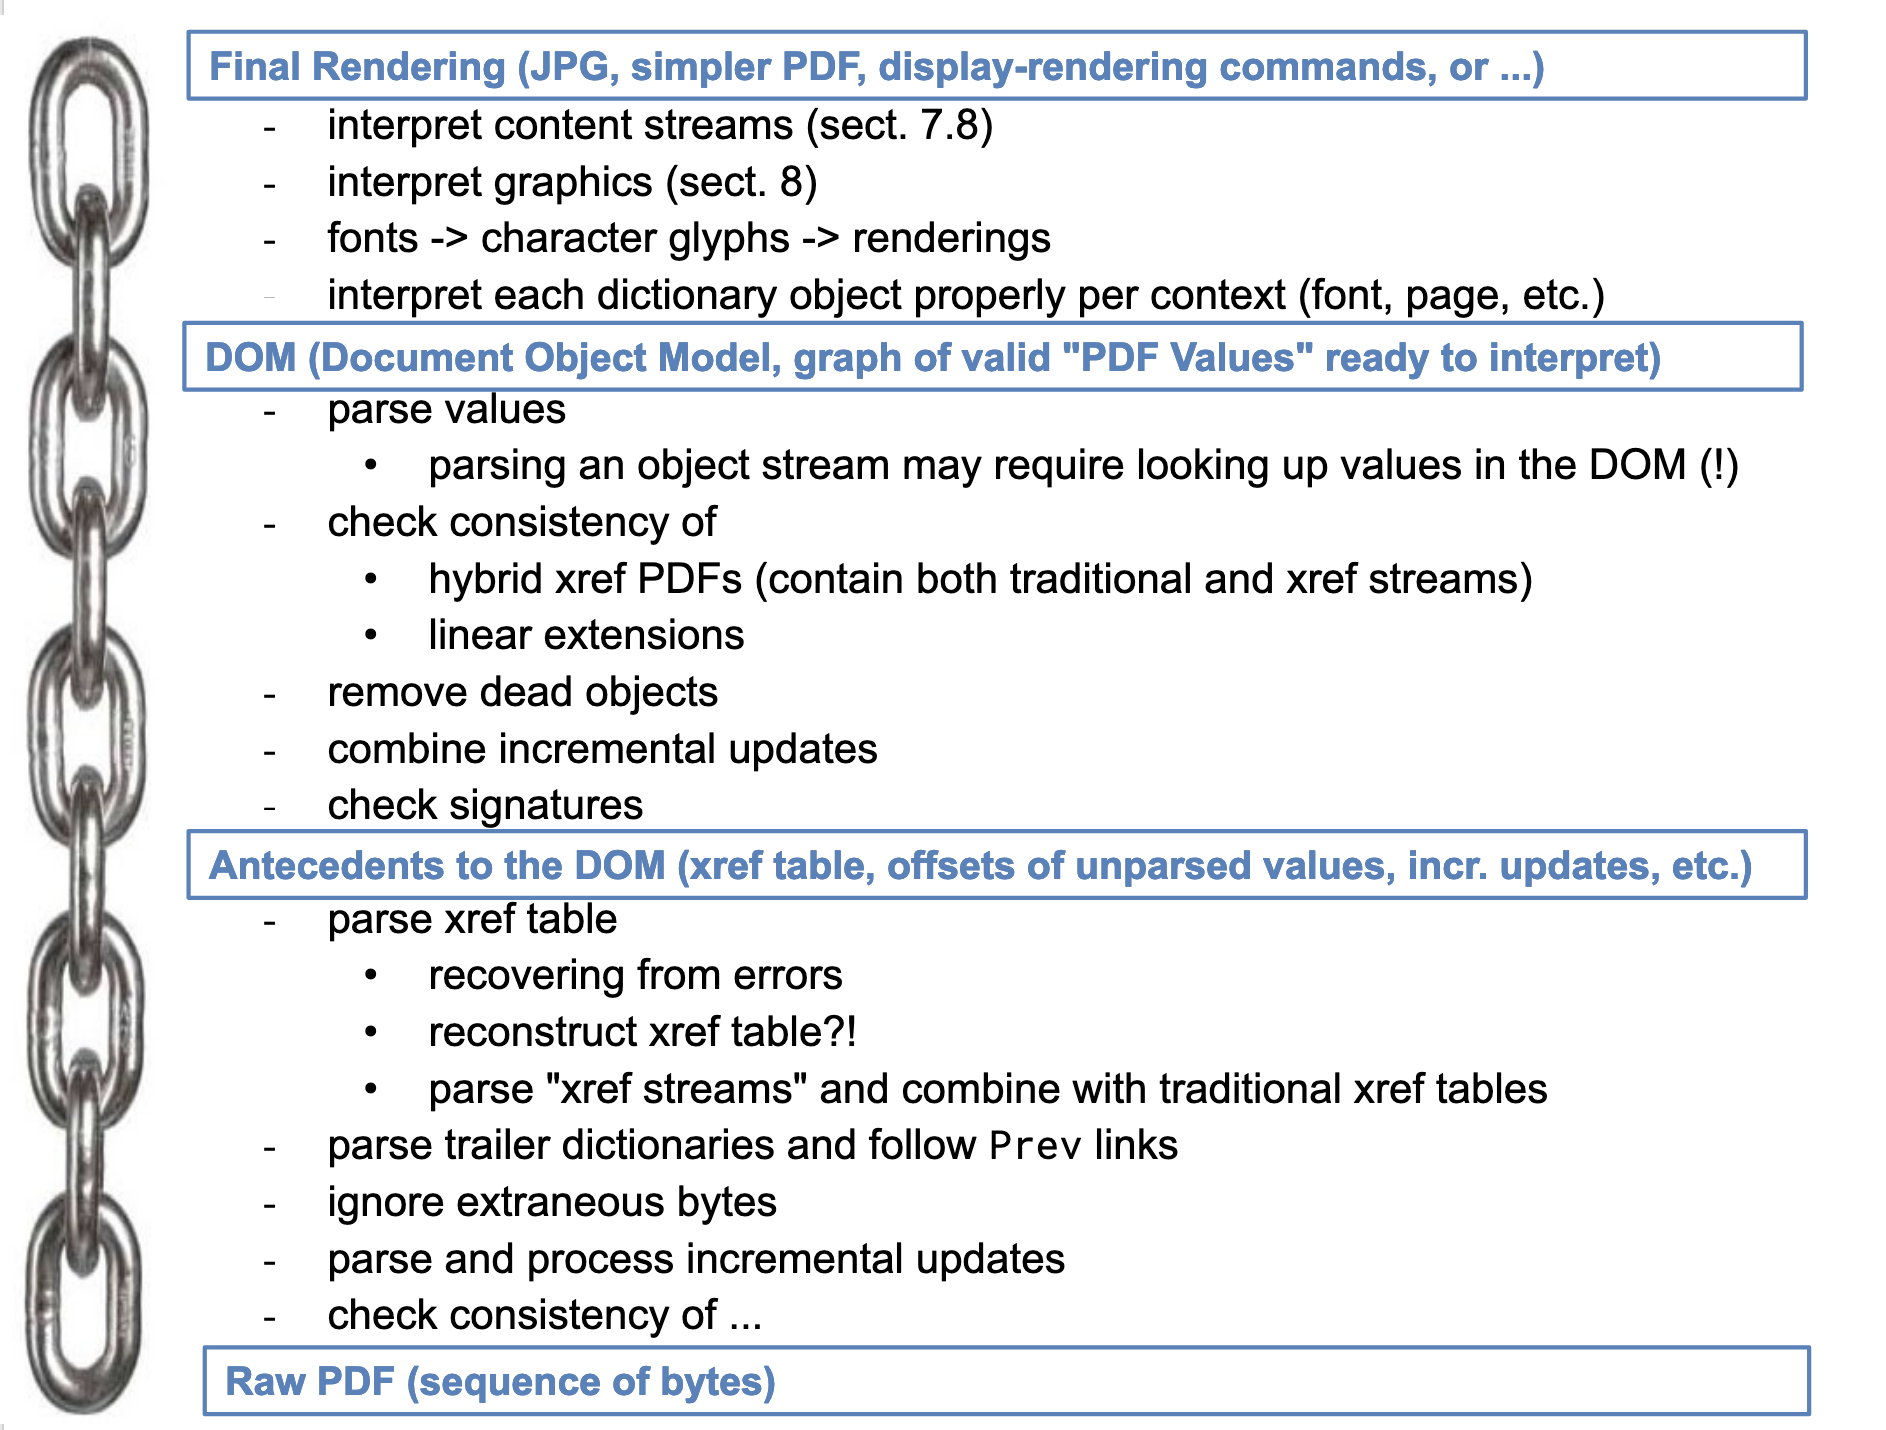
\includegraphics[width=0.8\linewidth]{figures/trustchain-diagram.png}
  \caption{Stages of PDF Parsing (the Trust Chain)}
  \mttodo{un-ascii-ify diagram}
  \label{fig:pdf-trust-chain}
\end{figure}

We have touched upon the complexities of parsing
PDF, but to appreciate these, one has to understand the
dependencies and interactions between the features.
In \cref{fig:pdf-trust-chain} we show the main stages diagrammatically.
To briefly sketch what's going on in each stage:
\begin{itemize}
\item Stage 1: Find and parse both the PDF header and the PDF trailer to locate
  the document trailer dictionary and the start of the last incremental update or
  the cross reference table of the original document in the case of no updates.
\item Stage 2: Find and parse each cross reference table or incremental update. 
  Note that this stage uses context from Stage 1 (such as the file offset and trailer
  information) in order to know  \emph{where} to start processing.
\item Stage 3: This stage does no further reading of the file, but computes the
   a XRef map of the final PDF by accounting for each set of edits performed by each incremental update.
   Incremental updates can add new objects, mark as free previous objects, re-instate previously 
   freed objects, and change context information in the trailer dictionary that 
   forms part of each incremental update.
\item Stage 4: Transform XRef map to object map. This stage is complex and
  requires three sub-stages, each of which does further file input and parsing.
  Further details are in \cref{sec:specifying}.
  If all goes well, we have a syntactically correct DOM.
\item Stage 5: Validate candidate DOM.  This stage takes the candidate DOM and
  semantically verifies that it represents a sensible Document Tree per the PDF Standard.
  E.g., each object in the DOM is well formed with required data types and values, 
  no unexpected recursion, etc.
\item Stage 6: Render DOM.  Here we render the validated DOM, or parts thereof,
  to the output format of choice.
\end{itemize}

Any error (malicious or otherwise) in an earlier stage will affect the output of stages that follow.
But note stages 2, 3, 4.1, 4.2, and 4.3 all depend on inputs from the previous stage to determine 
where and how to parse segments of the PDF input file.
Errors that percolate into these stages can
cause all forms of havoc (parsing wrong data, etc.).
%
The attentive reader will note that we have another instance of a \emph{Trust
Chain}.  The subsequent stages of the parsing process are \emph{completely
dependent} upon the earlier stages to properly parse and interpret the PDF
file.

An implementation \emph{might} merge stages 2, 3, 4.1, 4.2, 4.3 into
a single stage and give a \emph{semblance} of simplicity.
%
Our argument in what follows---particularly in
\cref{sec:single-pass-problems}---is
that such an implementation will be overly
complex and be a design for which it is highly intractable
to determine that it implements the standard
and to determine that it terminates for all input files.

We think it is important to understand PDF parsing in terms of this
\emph{Trust Chain} because
%
(1) it highlights the presence of the many ``dependent'' stages
in PDF processing;
%
(2) it highlights the importance of ensuring the pre-DOM parsing, data integrity relationships and
computation (the base of our Trust Chain) is correct and secure;
%
(3) it reminds us that the integrity of the DOM cannot be verified
independently of verifying all the earlier stages; and
%
(4) it illustrates that PDF parsing, although uniquely complex, is an instance of
a general concept.

Although \emph{Validate candidate DOM} (stage 5) might be considered tedious, the necessary checks are 
reasonably well defined by the bulk of the PDF Standard. Validation involves ensuring that each 
individual PDF object has all the required keys and appropriate values in the context of its reference in the DOM.
For example, a PDF object that is a thumbnail for a PDF needs to be an Image XObject and have a 
minimum set of required key names and their values each within predefined limits (e.g. both
\lstcd{Height} and \lstcd{Width} are required keys and must be non-negative integers). If the 
thumbnail reference in the candidate DOM is to a font dictionary or some other kind of
\emph{syntactically} valid PDF object then this is \emph{semantically} incorrect. Recent work
\cite{arlingtonPdfModel} created the first specification-derived comprehensive
machine-readable model of every object, their attributes and relationships in the PDF DOM. The use
of such a model for code generation, validation or test case generation can reduce the tediousness.


The \emph{Render DOM} stage also has many complications of its own, whether this be rendering a PDF
page to pixels for display or print, or extracting text contract, however for this paper we will
focus on stages 1-4.

We refer to stages 1 to 4 as pre-DOM parsing/computation; if anything
goes wrong pre-DOM---and lots can go wrong---there's hell to pay.
\todo{do we dare?!}

\todo{BH: I urge against: it's not so much that the tone is too
  risque, but (related) that it's not suitably precise.}


\section{PDF: Structure, Complexity, Vulnerabilities}
\label{sec:pdf}

\subsection{The PDF Format}
\label{sec:pdfstructure}

\begin{figure}[t]
    \centering
    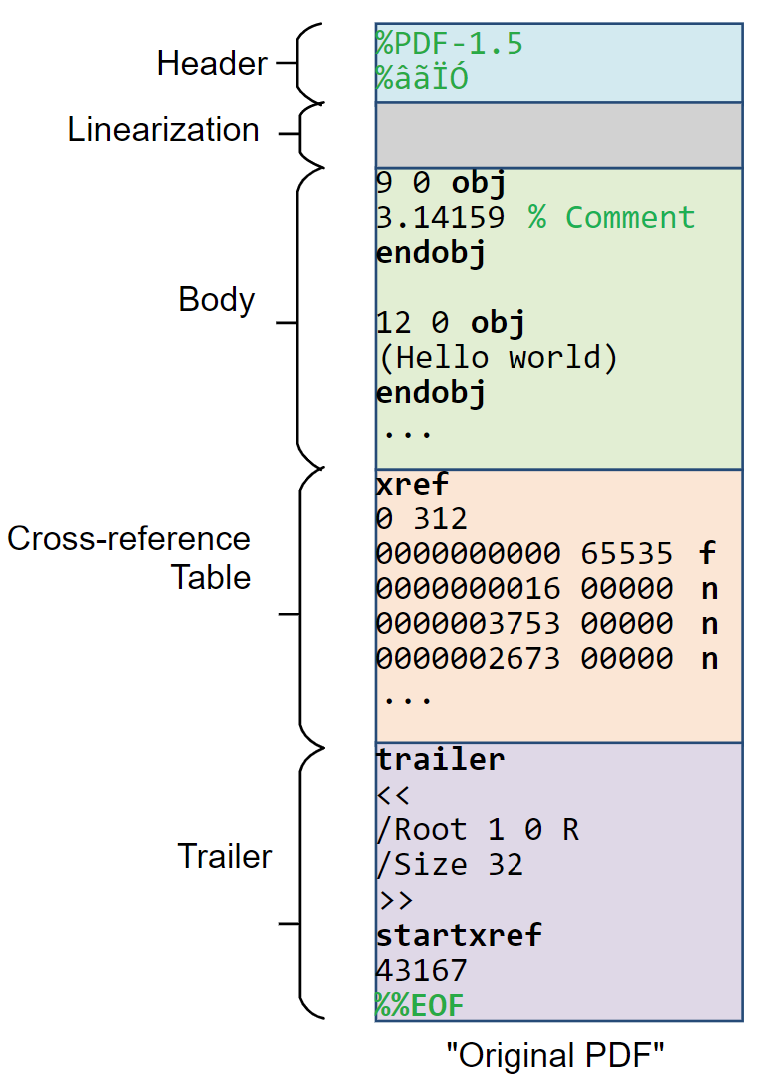
\includegraphics[width=0.65\linewidth]{figures/pdf-structure.png}
    \caption{The structure of a conventional PDF file: labeled sections with selections of representative grammar.}
    \label{fig:pdf-structure}
\end{figure}

PDF is a random-access file format that contains 8-bit binary data, line-based ASCII (7-bit)
text data (terminated with various end-of-line sequences), and a fixed format ASCII 
data format in different sections of a single file. The overall structure of a 
conventional PDF file without any incremental updates is shown in \cref{fig:pdf-structure} and 
described below, based on the official PDF ISO 32000 standard.
PDF 1.5 introduced more compact file structure capabilities known as cross-reference streams 
and object streams however, since this builds on the following concepts, this modern 
variation on the PDF file structure will be described later.

The PDF \emph{Header} section contains the file identification marker as an ASCII
text comment line \lstcd{\%PDF-} followed by the PDF version as single ASCII digits. 
An optional second comment line (starting with \lstcd{\%})
containing at least 4 bytes above 127 in value is recommended, to ensure 
that PDF files are not misidentified as purely 7-bit text files. 
All file offsets in PDF file are from the \lstcd{\%} sign in \lstcd{\%PDF-x.y}.  

The \emph{Linearization} section is an optional optimization section that enables what is commonly
known as ``fast web view''. This section must occur within the first 1024 bytes of a PDF and contains
data that enables a Linearized PDF aware parser to quickly display the opening page of a PDF
while the rest of a large PDF can download in the background.
Linearizatiom data is also invalidated by incremental updates (since an update might change objects
on the opening PDF page) and must therefore be checked and ignored.
%
Because not all PDF parsers support Linearization, it is a known form
of ``parser differential by design,'' where a \emph{parser
  differential} is a semantically meaningful difference in the result
of two parsers when run on the same document.
%
For the purposes of this paper, we will not consider Linearized PDF further.

The \emph{Body} section is where all indirect PDF objects are defined. Indirect PDF objects
are defined as those objects that have ``a unique object identifier by which other objects can
refer to it (for example, as an element of an array or as the value of a dictionary entry).''
Any PDF object may be defined indirectly: integers, real numbers, strings, arrays, dictionaries, 
streams, etc. Objects are defined by their object identifier (their object number and generation 
number pair) followed by the keyword \lstcd{obj}. 
The end of every object is defined by the keyword \lstcd{endobj}.
In \cref{fig:pdf-structure}, object 9 is a real number (in ASCII) followed by a comment
(introduced by \lstcd{\%}) and this is followed by object 12 which is a PDF literal string object
(enclosed in \lstcd{(} and \lstcd{)}).  
Every indirect object is reached by knowing the file offset to the start of the ASCII integer 
object number. This offset information for all indirect objects is stored in Cross-reference Tables.

The \emph{Cross-reference Table} section begins with the \lstcd{xref} keyword. For a PDF file
with no incremental updates, the next line will be a cross-reference sub-section text line comprising
two integers in ASCII (\lstcd{0 312} in this example). The first integer is an object identifier 
and in the case of an original PDF this must be 0. The second integer is the number of
objects in the cross-reference subsection.

There are two sets of
objects in every PDF document: the in-use list of PDF objects and a free list
of PDF objects. Object zero is always the start of the free list as it is not
otherwise a valid object number. Each incremental update may also move objects between these two sets.
In a conventional PDF, each entry for an object contains a fixed length 20-byte line of text.
The first 10 ASCII digits represent the byte offset to the object, followed by a single ASCII SPACE, 
followed by 5 ASCII digits representing an object generation number. This is then followed by
another single ASCII space and the keyword \lstcd{n} for in-use objects or \lstcd{f} for free objects.
Finally an end-of-line sequence is defined to ensure that the text line entry for each object has 
a 20-byte fixed length. A parsing subtlety is also that cross-reference sections are the only section 
in PDF where comments are expressly prohibited.

The \emph{Trailer} section is at the very end of every PDF file. 
It is defined as the end-of-file comment line \lstcd{\%\%EOF} immediately
preceded by the \lstcd{startxref} keyword followed by the file offset (in ASCII as a decimal) to 
the cross-reference table (i.e. the byte position of the \lstcd{xref} keyword 
from the the \lstcd{\%} of \lstcd{\%PDF-x.y}). Prior to this (but technically 
defined as being immediately \emph{after} the cross-reference table) is the trailer dictionary
identified by just the \lstcd{trailer} keyword, rather than the \lstcd{obj} and \lstcd{endobj}
keywords used in the PDF Body section.

\begin{figure}[t]
    \centering
    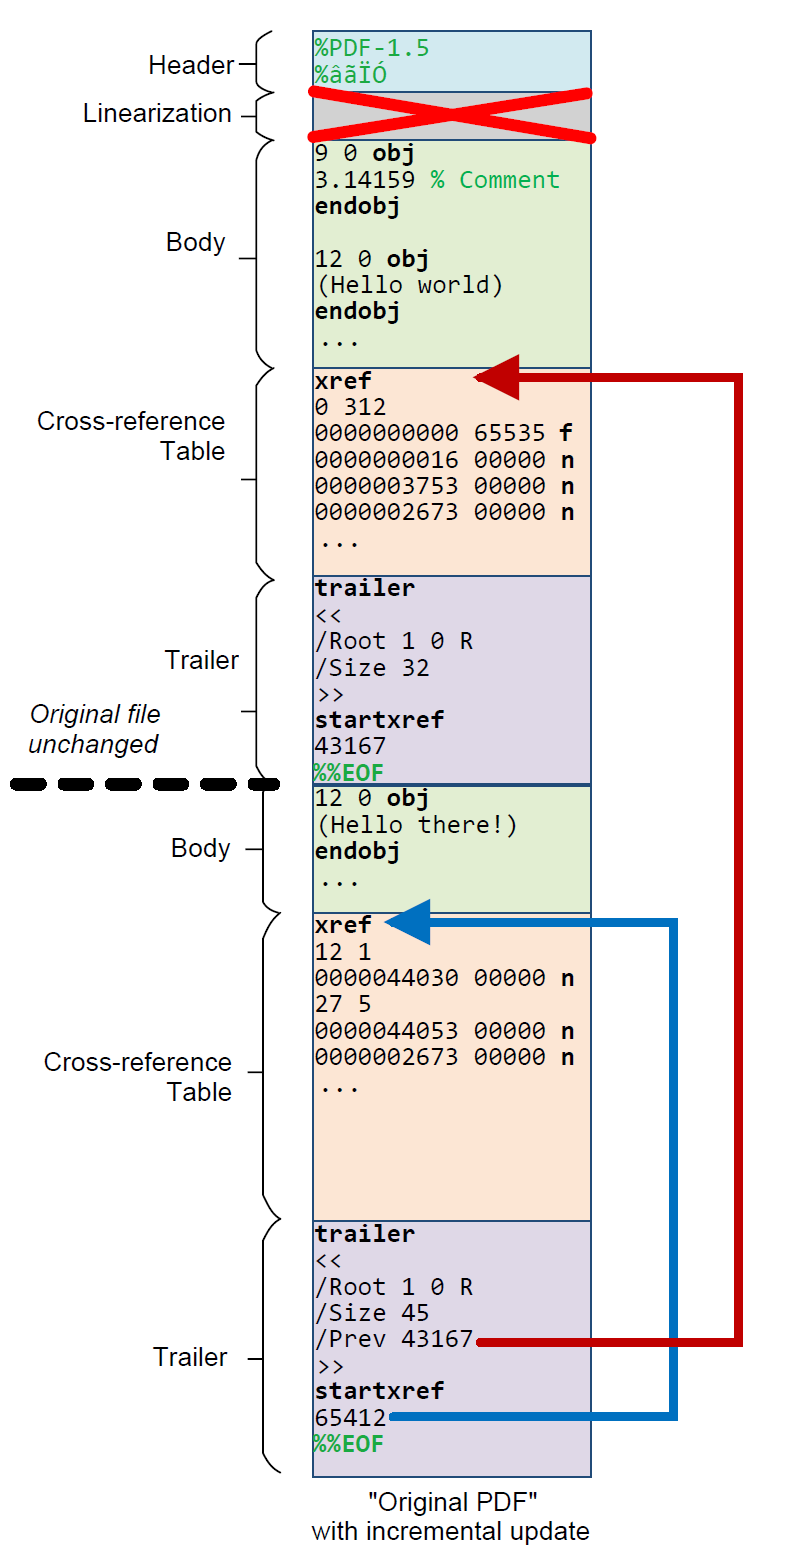
\includegraphics[width=0.65\linewidth]{figures/pdf-structure-incremental.png}
    \caption{Conventional PDF file structure with a single incremental update.}
    \label{fig:pdf-structure-incremental}
\end{figure}

As illustrated in \cref{fig:pdf-structure-incremental}, each incremental update will 
normally append a Body, Cross-reference Table, and Trailer sections
to a PDF file, with the entire original PDF remaining unchanged. The newly added incremental
update trailer dictionary must also contain information referencing the immediately 
previous cross-reference table by byte offset. The Body section of the incremental update 
will contain any new or redefined objects. If only fields in the trailer dictionary are updated then
a new Body section is not required. The cross-reference table for each incremental update
defines changes to objects made by that incremental update. This may include freeing
objects by adding them to the free list (the actual indirect PDF objects in
the PDF file are not actually deleted), and/or the addition of new objects. 

\begin{figure}[t]
    \centering
    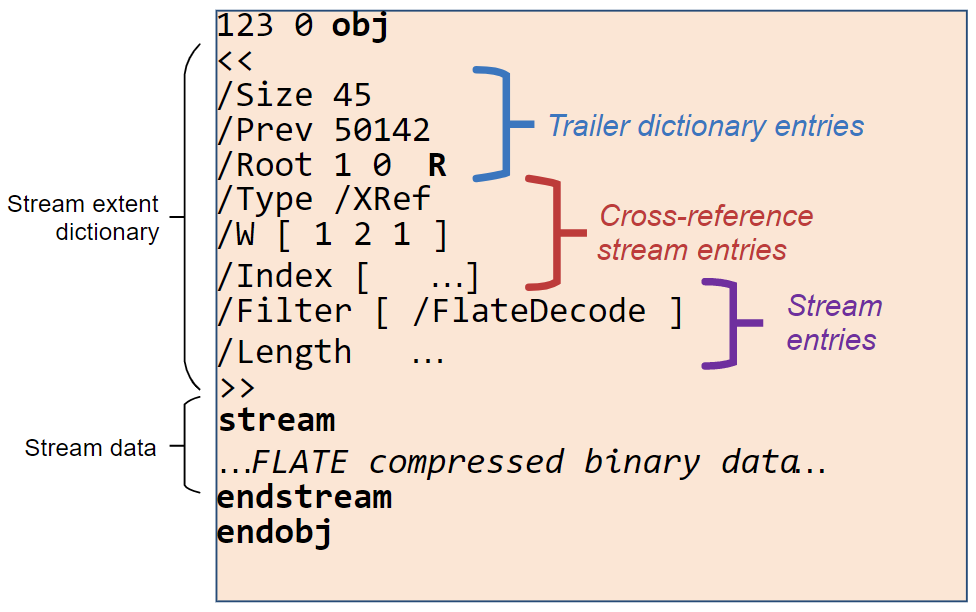
\includegraphics[width=0.65\linewidth]{figures/xrefstm.png}
    \caption{Example of a PDF 1.5 cross-reference stream.}
    \label{fig:XRefStm}
\end{figure}

As previously mentioned, PDF 1.5 introduced cross-reference streams and object streams as a means
to overcome physical file size limitations imposed by the 10-digit byte offset in the conventional
cross-reference tables.
Such files replace the Cross-Reference Table section (including the \lstcd{xref} keyword) 
with a PDF stream object containing binary data, as shown in \cref{fig:XRefStm}. 
Like all streams in PDF, cross-reference streams may also be compressed with algorithms such as FLATE 
to further reduce file size. If a cross-reference stream is used, then the trailer dictionary is also no
longer used. Instead the context-defining key/value pairs of the trailer are added to the stream 
extent dictionary of the cross-reference stream.

\begin{figure}[t]
    \centering
    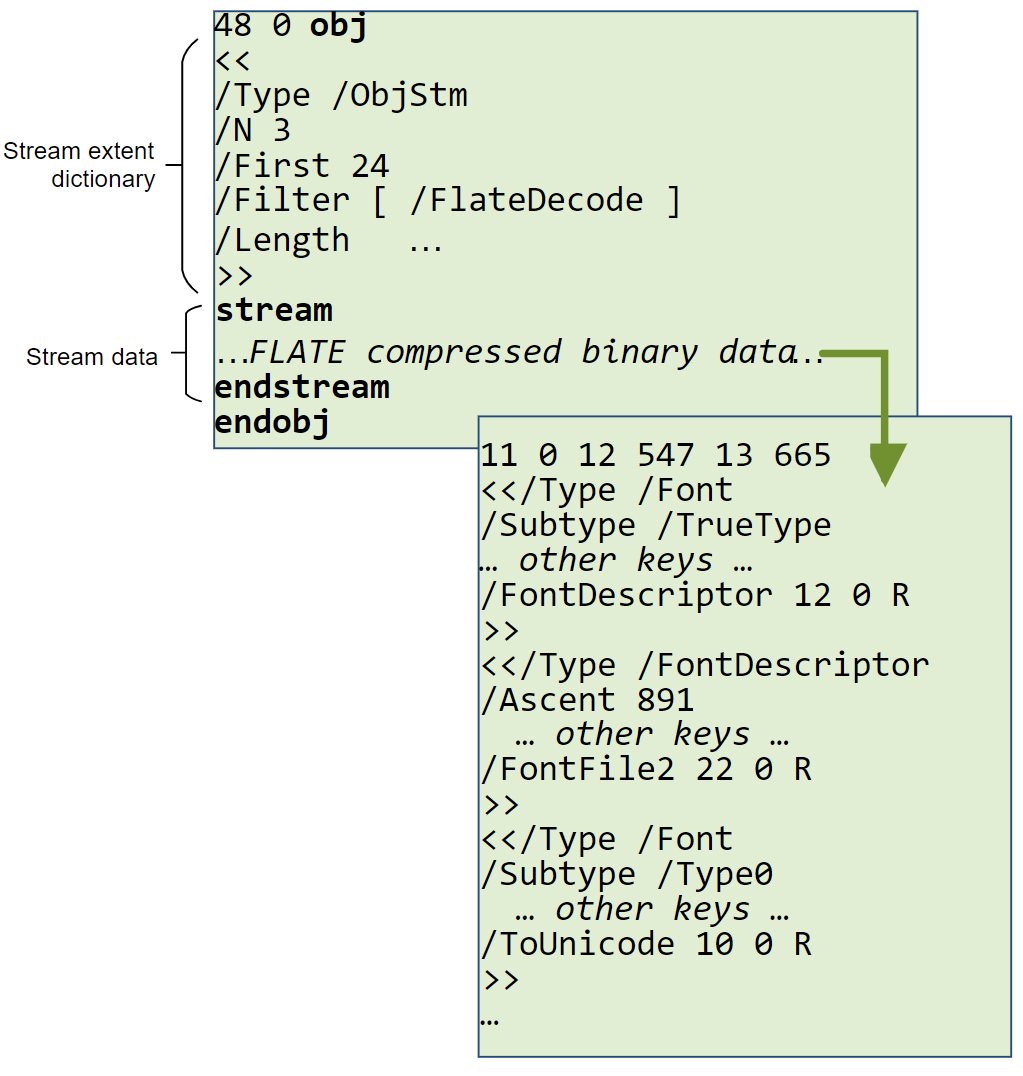
\includegraphics[width=0.65\linewidth]{figures/ObjStm.png}
    \caption{Example of a PDF 1.5 object stream and its uncompressed content.}
    \label{fig:ObjStm}
\end{figure}

Another optimization added by PDF 1.5 were object streams as illustrated in \cref{fig:ObjStm}.
It can be appreciated that a large PDF will
undoubtedly have many indirect objects and thus the repeated use of the object identifier pair with 
\lstcd{obj} and \lstcd{endobj} keywords can become a significant size burden. Object streams are
compressible text streams ``... in which a sequence of indirect objects may be stored, as an 
alternative to their being stored at the outermost PDF file level''. 
Syntactically object streams no longer uses the \lstcd{obj} and \lstcd{endobj} keywords and replace 
the object identifier pair with a single object number and a byte offset within the object stream. 
By using stream compression algorithms, this ASCII text data can be drastically reduced in size.
If object streams are used, then cross-reference streams must also be used. However cross-reference 
streams may also be used by themselves with the conventional Body section.

As noted above because both cross-reference streams and object streams are standard PDF streams, they 
can benefit from stream compression. However this also means that parsers are   
susceptible to ``ZIP bombs'' \todo{explain!} attacks, cycles in object references, and handling of semantic errors (invalid stream extent dictionaries) 
during pre-DOM processing!

A further complication is the concept of ``hybrid-reference'' PDF files, where both conventional cross-reference tables and cross-reference streams co-exist in the same PDF so as to provide some semblance of support for non-PDF 1.5 aware parsers. This complication is not addressed further in this paper.

There is no limit to the number or types of incremental updates that can be added to a PDF file. Later
updates may also ``undo'' changes from any previous incremental updates by restoring (changing back to in-use)
previously feed objects. For incremental updates, PDF object numbering 
does not have to be sequential, with skipped object numbers assumed to be on
the free list (although this is not stated explicitly in the PDF standard).

In effect, incremental updates form a timeline of all changes made to a PDF, with parsing starting
at the end of the file with the most recent change back to the original document at the to of the file.

\subsection{Root Causes of PDF Complexity}
\label{sec:rootcause}

Most data formats can be described by much simpler mechanisms;
most language processors (e.g., a Python parser) can be described and parsed by
textbook methods (e.g., \emph{lex} and \emph{yacc} are sufficient for
most language processors);
so what makes PDF processing so much more complex?

As described above, PDF uses random access to byte offsets to then parse lines of text,
which may then switch to binary data or fixed-length record parsing. 
In some, but not all, cases the end of an object can be known apriori, but in the most common case 
of conventional cross-reference tables, only forward parsing can determine the end of an object. 
This gives rise to a phenomena we call \emph{cavities} where not every byte in a PDF file is parsed.
Such cavities can be used to hold data in an alternate format giving rise to polyglots, or potentially
to hold shellcode that might be na\"ively loaded into memory and further exploited 
in vulnerable parsers.
In addition, various descriptions in the PDF standard require ``parsing backwards'' which is 
an unnatural programming language idiom. Furthermore, some explicit pre-DOM requirements
in the PDF standard
refer to bytes \emph{before} a given byte offset and that parsers are highly unlikely to check. 
Our investigations reveal that these requirements are effectively ``writer requirements'' (unparsers) to
support better file reconstruction and recovery in the event of later data corruption. 
However if these requirements are never checked or enforced then it is possible to use them as attack
vectors.  
The PDF specification also requires multiple
sublanguages and computation (such as stream decompression).

If a PDF file accidentally or maliciously fails to adhere to this set of complex PDF file structure
rules, or an implementation has bugs, PDF parsers will typically silently attempt to recover
by reconstructing the cross-reference table information. 
This is not defined by the PDF file format standard so 
ad-hoc algorithms are used. Typical reconstruction algorithms parse from the start of a PDF 
file, searching for indirect PDF objects (\lstcd{x y obj ... endobj}) at the start of lines. This can clearly result
in ambiguous reconstruction of a PDF DOM and is highly likely to lead to parser differentials.

The PDF DOM created by a set of indirect PDF objects forms a directed graph. 
Each PDF object is a vertex and indirect references between objects form the directed edges. It is 
specifically \emph{not} acyclic as PDF formally defines concepts such as parent references to 
pages and other objects. This is different to most XML-based file formats because XML naturally 
forces hierarchical relationships via nesting of tags.

The PDF standard defines very few explicit data integrity relationships for pre-DOM parsing. 
Our work has been to critically review the under-appreciated and under-studied pre-DOM PDF
file structure using formal methods to highlight data integrity relationships that can 
ensure the PDF Trust Chain is robust prior to DOM processing.

% ------------------------------------------------------------------------------
\subsection{Vulnerabilities}
\label{sec:vulnerabilities}

% As will become even more apparent, there is a significant amount of
% parsing and computation that needs to be done \emph{pre-DOM}.

The majority of prior work researching PDF vulnerabilities start with a pre-existing PDF DOM,
ignoring pre-DOM parsing and processing~\cite{smutzMaliciousPDFDetection2012,liuDetectingMaliciousJavascript2014,iwamotoStudyMaliciousPDF2016}. 
This work typically looks for obfuscated PDF objects such as
JavaScript streams or strings, action objects, URL strings, or file attachment objects that 
can lurk in various places throughout the PDF DOM. Machine-learning approaches so far have not  
used feature vectors based on the contextual information in PDF pre-DOM file structure~\cite{andrewmangleAnalysisMachineLearning2021,manharmohammedHAPSSAHolisticApproach2021}. 
Prior work in privacy has identified that incremental updates obviously pose a risk for complete
redaction and data scrubbing workflows if not processed correctly~\cite{adhataraoHowArePDF2021,y.fengSystematicMethodPDF2018}.
Given our recent points about the \emph{PDF Trust Chain}~\cref{sec:trust-chain}, it should not 
surprise us that some PDF attack vectors involve aspects of breaking the \emph{DOM} abstraction.
I.e., the root cause occurs pre-DOM.

{\bf{Supply Chain attacks}} are a generalization of {\bf{Shadow Attacks}} which were coined by Mainka 
et al.~\cite{mainkaShadowAttacksHiding2021} whereby an attacker infiltrates a workflow and 
maliciously manipulates a document in some way. This manipulation may be entirely syntactically valid.
Only later in the workflow, possibly after a 
digital signature is applied or an official approval step, the malicious data is 
activated. In the case of digitally-signed documents, this severely undermines confidence and trust
in digital signature technology.

\todo{at this point, have we defined parser differentials and polyglots? 
"Parser differential" is bottom of page 2, but NO for polyglot - it's a little below }
\todo{we are using both 'parser differential' and ``ambiguous'': use one. 
They are different but related: In the intro we define ambiguities as ONE cause of parser 
differentials. In the PDF section I already wrote about "differential by design" caused 
by Linearized PDF. Is a parser differential necessarily something that a human can see? 
I would assert it is as you define below - so an ambiguity can also lead to a vuln which 
may not be noticeable (secret leak, etc). }

{\bf{Parser Differentials}} are a real threat as attackers leverage differences in output
to present different information to different individuals, where the individual might be a human
or a machine. Parser differentials arise due to a combination of parser weaknesses, 
parser permissiveness, ambiguities, and unexpected input. In the case of PDF pre-DOM file structure, we have been
able to easily demonstrate parser differentials  
\todob{put small example here or ...? Could reference this PoC: https://github.com/pdf-association/safedocs/tree/main/Miscellaneous%20Targeted%20Test%20PDFs#dual-startxrefpdf
or the vuln we discovered that is quoted back in the intro }

{\bf{Polyglots}} are a potential threat in any system or workflow which relies on different parsers
at different stages. If a firewall product determines a file to be of file type \emph{X} and then only 
scans for vulnerabilities relevant to file type \emph{X}, but later software decides the same file 
is file type \emph{Y}, an organization is then vulnerable.
Polyglots arise from the creative use of cavities, permissive implementations, 
and other blind spots in a file format specification where arbitrary data can be placed 
that does impact processing (e.g. in comments or strings, in freed or unreferenced objects, etc.).

{\bf{Denial of Service (DoS)}} is of increasing concern to the PDF industry, with many PDF services
and products utilizing cloud-based processing. In cases like large-scale automated invoice 
processing, DoS attacks can also incur additional expenses as well as inconvenience for an organization 
as exception-handling by human operators may be invoked.  

It should also be no surprise that due to the complexity and subtleties of the PDF standard described above,
extant data exhibits many errors in cross-reference tables and related pre-DOM context information.
To date, there has not been a comprehensive analysis of PDF file structure faults in extant data
caused by defects in PDF writers. One core reason is that dedicated tooling is lacking that reliably reports
all technical variations from the PDF standard. However analysis of open-source PDF parser code bases
does highlight tools with varying degrees of lightweight reporting, however all exhibit permissive features related
to pre-DOM processing:

\begin{itemize}
    \item deviation from the required 20-byte fixed cross-reference table entry, with support for
    19- and 21-byte variations due to additional white space or incorrect line endings;
    \item errors in byte offsets to indirect PDF objects and objects in object streams;
    \item errors with \lstcd{startxref} byte offsets;
    \item incorrect trailer dictionary data (such as \lstcd{Size}), leading to implementation-dependent decisions;  
    \item terminating pre-DOM processing prematurely (i.e. not processing all incremental updates and  
    being susceptible to Shadow Attacks).
\end{itemize}


\section{Specifying the PDF DOM's Foundations}
\label{sec:specifying}

This section %
states our goals in producing a formal partial definition of PDF
(\Cref{sec:spec-goals}) and then presents the specification's core
definitions (\Cref{sec:core}), followed by its definitions of each
stage of the PDF Trust Chain (\Crefrange{sec:stage-1}{sec:stage-4}).
%
\Cref{sec:assessing} analyses the resulting specification.

\subsection{Specifying PDF: Goals and Approach}
\label{sec:spec-goals}

% REMEMBER terms: complies with standard, compatible with
Ideally, a PDF implementation should:
\begin{itemize}
\item comply with the PDF standard,
\item when not fully supporting the standard, do so gracefully,
\item support common PDF malformations
  to be compatible with extant PDFs, but \emph{without} introducing ambiguities
  or causing other unintended consequences (we refer to this as \emph{permissiveness}),
\item and all the while, contain minimal bugs, robustly cope with unexpected input and stay resilient
  against all attacks.
\end{itemize}
Achieving the above is challenging due to many factors:
\begin{itemize}
\item The intrinsic complexity of PDF:
  PDF is a \emph{less than ideal} design that reflects almost 30 years of
  an evolving standard.
  %
  PDF has multiple redundant features and is explicitly designed to facilitate efficient processing of
  large files (``efficiency hacks'').
  %
  PDF involves multiple sublanguages (dialects) and embedded formats.
  %
  PDF contains complex parsing needs, such as backwards searching and
  embedded file offsets.
\item Lack of formality in the standard. Thus, implementators
  need more effort to understand it and comply with its intentions.
  Implementations commonly over implement, under implement,
  and wrongly implement the standard.
  Because writing a rewriting  PDF implementation from scratch is a significant and costly effort,
  implementors are incentivized to patch existing code (correct or not).
\item The standard primarily defines just one thing: \emph{what is a valid PDF file},
  with only a few processor requirements. Many technical details are also delegated to the numerous normative references.
  This leaves the majority of decisions up to each implementation:
  (1) What should absolutely \emph{not} be allowed (because in the real world
    implementations are more or less relaxed)? And similarly,
    what are deemed to be acceptable, reasonable error recovery methods?
  (2) What is required to support backwards and forwards compatibility?
  (3) What is done when redundant features are inconsistent with one
    another: which, or neither, has priority?
    Similarly, what is done when the stated PDF version and the PDF
    constructs used don't match?
  (4) What is \emph{required} from the PDF writer versus
    what do we \emph{require} the PDF reader to check?
  (5) Behavior when given in incorrect PDF.
\end{itemize}

Failure to faithfully implement the standard can result in ambiguities
between implementations, parser differentials as well as direct vulnerabilities (such as
Shadow Attacks or DoS attacks).

\mtnote{this last, (5), seems pretty key and
  feels like a major omission in the standard! If the answer is
  yes, then there's nothing keeping an implementation from only
  doing enough to ``work on good pdfs'' without even checking that it
  IS a good PDF.  Thus, we have the tool that only reads the 'e'
  in ``endobj''.  Is this reasonable?  Are there vulnerabilities that
  would exist in such implementations?
}

% define formal specification:
A \emph{formal specification} of a format does not immediately resolve
all of the above issues, but it is a critical artifact for clarifying
the standard, understanding the vulnerabilties, and aiding
implementors of PDF processors.
%
In this work, we have produced a specification of one component of PDF
in the Haskell programming language~\cite{jones2003haskell}.
%
A detailed presentation of Haskell's features is beyond the scope of
this paper, so we note only that it is a statically typed, pure,
functional programming language with a lazy;
%
we review its other features throughout the paper when they are
relevant.

% say more about the spec's scope:
The scope of our specification is the gap between the low level
parsers (parsing integers, parsing XRef entries, etc.) and the
processing that happens after the DOM is created (stages 5 and 6).
%
I.e., stages 1--4.
%
Primitive parsers are assumed, not included in this spec, as other
formalisms, such as the \emph{DaeDaLus Data Description
  Language}~\cite{daedalusrepo}, are better suited to specifying the
primitive parsers.
%
See \cref{sec:appendix1} for a list of the primitive parsers
with their type signatures.
%
The full specification of DaeDaLus is publicly available
online~\cite{daedalusrepo}.

\begin{itemize}
\item Our specification is formal and executable (though not
  necessarily efficient).
  %
  We already have the PDF standard: which is not always clear, not always
  consistent. 
  This is our motivation for choosing Haskell over English prose or
  pseudo-code or other informal approaches.
  For the reader
  without a reading knowledge of Haskell, we understand that parts of
  the specification could be a little obscure, but our hope is that a
  precise, formal specification may prove to be more useful than
  pseudo-code or the like!
  
\item Our specification is purely functional: no ad hoc global variables are
  hidden, the data-dependencies in the spec fully represent all the
  data-dependencies.  Motivated by the Trust Chain issues
  (\cref{sec:trust-chain}), our objective was to capture all dependencies.
  
\item Our specification hides no difficulties: one could implement a PDF parser
  by writing the omitted functions, but the spec stands complete, as
  is!
  % \footnote{One caveat: the addition of support for \emph{some} features
  % could require some re-design.  E.g., signature validation, as discussed in
  % \cref{sec:updates-and-signatures} would require non-trivial changes.
  % }
\end{itemize}

This spec supports PDF 2.0, including compressed objects and XRef streams.
%
It (safely) ignores linearization data, and in hybrid XRef PDFs
it ignores the traditional \xref{} tables designed for pre PDF 1.5 readers.
It processes signatures (as incremental updates) but it does not support
validation of signatures.

%%%%%%%%%%%%%%%%%%%%%%%%%%%%%%%%%%%%%%%%%%%%%%%%%%%%%%%%%%%%%%%%%%%%%%
\subsection{Core definitions}
\label{sec:core}
%%%% begin: Hs code not in paper %%%%
\iffalse
\begin{code}
{-# LANGUAGE EmptyDataDecls, TypeOperators, LambdaCase #-}
module Spec where
import           Control.Monad
import           Data.Char
import           Data.Foldable(foldlM)
import qualified Data.IntSet as IntSet
import           Data.List
import qualified Data.Map as M
import           Data.Map(Map)
import           Types
import           Utils
import           Primitives
import           Streams
\end{code}
\fi
%%%% end: Hs code not in paper %%%%

\lstcd{pPDFDom} (\cref{fig:spec}) implements stages 1 through 4 (illustrated in \cref{fig:pdf-trust-chain}).
% 
\lstcd{pPDFDom}'s type (line 1) denotes that it
is a \emph{monadic} parser \lstcd{P} that returns a value of type
\lstcd{DOM}.
%
In general, monads are a rich class of parameterized types that
describe a surprising variety of data and computations.
%
For the purposes of this paper, it suffices to view a monad as a container that provides an operation to sequence effectful \emph{actions} (specifically, functions from some type to a monad over a potentially distinct type) in a purely functional manner;
%
effects can be global variables (or mutable state), exceptions, I/O, and etc.

% do notation:
Haskell provides a syntactic form for concisely sequencing actions, structured as the keyword \lstcd{do} followed by bindings of the form \lstcd{x <- A}, which denotes that the action \lstcd{A} is performed and its resulting value is bound to variable \lstcd{x} to be used by further actions.
%
E.g.,
\begin{codeNoExecute}
  topAction :: P Int
  topAction = do
              result1 <- action1 args1...
              let x = <PURELY-FUNCTIONAL-EXPRESSION>
                  f x = <FUNCTION> -- not an action
              result2 <- action2 result1 args2...
              return (anyPureFunction result2)
\end{codeNoExecute}
%
\todo{do we really need this extra example? Can't we just point to Fig. 6?}

% walk through P:
The specific parser monad \lstcd{P} abstracts effects on a parser's state.
%
Its state includes %
\textbf{(1)} one read-only variable, which stores the PDF file being read, and %
\textbf{(2)} one mutable variable \rdloc{}, which stores the offset in the file at which the next byte is read.
%
\rdloc{} is accessed by primitive parsers (which have type \lstcd{P})
and is updated by sequencing the parsing action
\begin{codeNoExecute}
  seekPrimitive :: Offset -> P ()
  seekPrimitive off = <update readLocation with 'off'>
\end{codeNoExecute}
%
\mttodo{readLocation equals \rdloc{}?}
%
\texttt{P} parsers implicitly track parsing errors, which are thrown when an input document is not in the defined format.
%
I.e., each parsing action of the form \lstcd{x <- A} can be viewed as attempting to parse according to action \lstcd{A}, binding a result to variable \lstcd{x} only on success and failing otherwise.

% type annotations:
To aid understandability, expressions are occasionally annotated with types (see \cref{fig:spec} lines 8, 11, and 14).

\begin{figure}[t]
\centering
\lstset{numbers=right}
\begin{code}
pPDFDom :: P DOM
pPDFDom =
    do
    -- Stage 1:
    (seek,xrefOffset,version) <- findHeaderAndTrailer
    -- Stage 2:
    updates <- parseAllIncUpdates seek xrefOffset
               :: P [(XRefRaw, TrailerDict)]
    -- Stage 3: combine all the updates to get a single xref table
    xrefs <- combineUpdates seek updates
             :: P (Map ObjId (Offset :+: Type2Ref))
    -- Stage 4:
    dom <- transformXRefMapToObjectMap seek xrefs
           :: P DOM
    -- final checks and validations:
    finalValidations dom version updates
    return dom
\end{code}
\caption{A formalization of pre-DOM stages 1--4 in Haskell.}
\label{fig:spec}
\end{figure}


%%%%%%%%%%%%%%%%%%%%%%%%%%%%%%%%%%%%%%%%%%%%%%%%%%%%%%%%%%%%%%%%%%%%%%
\subsection{Stage 1: find and parse the header and trailer}
\label{sec:stage-1}

% give the code for stage 1:
Stage 1 is defined as follows:
\begin{code}
findHeaderAndTrailer :: P (SEEK, Offset, Version)
findHeaderAndTrailer =
    do
    -- find "%PDF-x.y" near start of file, searching the first 1000 bytes:
    (version, headerOffset) <- findPDFHeader 1000

    -- search backwards from EOF for 'startxref', gives up after 1001 bytes:
    xrefOff <- findStartxrefThenParseToEOF 1001
    
    let seek n = seekPrimitive (headerOffset+n)
    return (seek, xrefOff, version)
    
type SEEK = Offset -> P () -- type of seek
\end{code}

Neither of the magic numbers $1000$ or $1001$ used in the definition are specified precisely
by the PDF standard, which requires only that they be numeric values
that are ``reasonably small'' \todo{is this a quote from the standard? How did we pick 1000 and 1001?}.
%
This is an immediate cause of ambiguity in the standard (and thus an
invitation for \pd{} in conformant document processors).

File offsets in a PDF are not defined in relation to the beginning of
the file, as might be expected, but instead to the beginning of the
\emph{PDF header};
%
the \lstcd{seek} provides a clean abstraction that defines this
aspect.
%
But we will need to pass \lstcd{seek} to all the actions that need to
``seek'' in the PDF file (note this being done in \cref{fig:spec}).

Because the two function calls (lines 5 and 8) have no data
dependencies, they can be performed in any order.
%
\haskellnote{The spec has no global variables beyond \rdloc{} and neither function
  depends on it.}

The full definition of \lstcd{findStartxrefThenParseToEOF} is
omitted, to simplify the presentation.
%
In abstract terms, it:
\begin{enumerate}
\item Finds the ``EOF marker'' \lstcd{\%\%EOF} (near the end of the physical
  file);
\item Parses ``backwards" to find the last \lstcd{startxref} keyword
  followed by an end-of-line sequence;
\item Parses the integer value encoded as a sequence of ASCII bytes
  (this represents the byte offset in the PDF file, which as noted
  above is adjusted for any preamble to the Header).
\end{enumerate}

%%%%%%%%%%%%%%%%%%%%%%%%%%%%%%%%%%%%%%%%%%%%%%%%%%%%%%%%%%%%%%%%%%%%%%
\subsection{Stage 2: Find and Parse Incremental Updates}
\label{sec:stage-2}
%
Stage 1 only finds the start of trailer;
%
the trailer dictionary itself, along with the complete cross-reference table, are defined in stage 2 as follows:
%
\lstset{numbers=right}
\begin{code}
type Update = (XRefRaw, TrailerDict)

pIncUpdate_Traditional :: SEEK -> P Update
pIncUpdate_Traditional seek =
    do
    (xrefRaw, xrefEndOff) <- pXrefRaw :: P (XRefRaw,Offset)
    validate \$
      verifyXrefRaw xrefRaw
        -- this ensures no duplicate objectIds
    seek xrefEndOff
       -- This seek is needed because pXrefRaw doesn't need to read
       -- the entries of each XRef subsection, so let's leave the
       -- current file read location after the xref table.

    pSimpleWhiteSpace -- no comments allowed between XRef table and ..
    keyword "trailer"
    trailerDict  <- pDictionary
    trailerDict' <- dictToTrailerDict trailerDict
                    -- ensures dictionary has proper keys
    return (xrefRaw, trailerDict')
\end{code}
\lstset{numbers=none}

\lstcd{validate} (line 7) is a special function used to demarcate semantic checks (line 8) that are not necessary to
create the DOM but which could detect invalid or inconsistent PDFs.
%
The check could be used in a ``validate'' mode, but would not necessarily be performed by all implementations.

% produces unparsed xref table subsections:
The resulting subsections of the \xref{} table are unstructured, each of type \lstcd{XRefRaw}, rather than a sequence of fully parsed \xref{} entries;
%
this aspect of the definition is revisited and fully motivated in \Cref{sec:stage-3}.
%
The partially structured representation still retains a set of \objid{}'s and for each, the offset of its of its \xref{} entry.
%
Constructing the representation critically relies on a precise requirement established in the standard: an \xref{} entry must have exactly 20 bytes.

The \xref{} table and trailer themselves are simply instances of incremental updates, which are parsed as follows:
\lstset{numbers=right}
\begin{code}
parseAllIncUpdates :: SEEK -> Offset -> P [Update]
parseAllIncUpdates seek offset =
  parseAllIncUpdates' IntSet.empty seek offset

parseAllIncUpdates' :: IntSet.IntSet -> SEEK -> Offset -> P [Update]
parseAllIncUpdates' prevSet seek offset =
    if offset `IntSet.member` prevSet then
      error "recursive incremental updates"
    else
      do
      seek offset
      (xref,trailerDict) <- pIncUpdate seek
      case trailerDict_getPrev trailerDict of   -- lookup 'Prev' key
        Nothing      -> -- no Prev key, we're done:
                        return [(xref,trailerDict)]
        Just offset' -> -- Prev key found, find updates starting at
                        -- offset':
                        do
                        us <- parseAllIncUpdates'
                                (IntSet.insert offset prevSet)
                                seek
                                offset'
                        return ((xref,trailerDict):us)
\end{code}
\lstset{numbers=none}
%
Much of the above definition is dedicated to ensuring that potential loops in the \lstcd{Prev} offsets do not cause the definition to lose well-foundedness (or in operational terms, that the natural corresponding parser does not loop infinitely).
%
The set \lstcd{prevSet} tracks the offsets of every update processed.
%
The definition %
\textbf{(1)} \lstcd{seek}s to the \lstcd{offset} and parses the update, then 
\textbf{(2)} checks for a \lstcd{Prev} key.
%
If no key is present, then parsing is complete;
%
otherwise, parsing continues with an extended set of offsets.

% supporting xref tables:
\lstcd{pIncUpdate} supports \xref{} tables as defined in versions of PDF up to 1.5 and represented using cross-reference streams:
\begin{code}
pIncUpdate :: SEEK -> P (XRefRaw,TrailerDict)
pIncUpdate seek =
      pIncUpdate_Traditional seek
  .|. pIncUpdate_XrefStream seek
      -- I.e., parse one or the other,
      -- syntactically, they are mutually exclusive.

pIncUpdate_XrefStream :: SEEK -> P (XRefRaw,TrailerDict)
pIncUpdate_XrefStream seek = notImplementedYet
\end{code}
%
The function \lstcd{pIncUpdate_XrefStream} is more
complex than \lstcd{pIncUpdate_Traditional} but the resulting
data is equivalent.
%
It also determines subsections without parsing the \xref{} entries.

% recap:
Upon success, stage 2 produces values from which a client can directly determine all \objids{} in the PDF and produce the trailer dictionaries and incremental updates.
%
The only PDF values that have been parsed are trailer dictionaries, but many documents can be rejected, including those with recurring \objids{} in the \xref{} tables.
\mtnote{check this phrasing}

%%%%%%%%%%%%%%%%%%%%%%%%%%%%%%%%%%%%%%%%%%%%%%%%%%%%%%%%%%%%%%%%%%%%%%
\subsection{Stage 3: combine incremental updates}
\label{sec:stage-3}
%
In stage 3, updates are processed from last to first:
\begin{code}
combineUpdates :: SEEK
               -> [(XRefRaw, TrailerDict)] 
               -> P (Map ObjId (Offset :+: Type2Ref))
combineUpdates seek updates =
    do
    let (xref,dict):us = updates -- safe because: null(updates)==False

    -- parse all xref entries in last (near EOF) update:
    xrefEntries <- mapM (thawXRefEntry seek xref) (getObjIds xref)

    -- initial Map:
    let tbl0 :: Map ObjId XRefEntry
        tbl0 = M.fromList xrefEntries

    -- merge each update into tbl0:
    tbl1  <- foldlM (mergeUpdate seek) tbl0 us
    return (removeFrees tbl1)

type XRefEntry = Free :+: (Offset :+: Type2Ref)
\end{code}

Each incremental update can add new objects, mark existing objects in use as free, or update objects.
%
\lstcd{XRefEntry} is defined to process updates from last to first;
%
it could have been defined alternatively to parse \xref{} entries only as needed.
%
\todo{why did we choose the option that we did?}

\todo{say what mergeUpdate does, informally}

\begin{code}
mergeUpdate :: SEEK
            ->  (Map ObjId XRefEntry)
            -> (XRefRaw, TrailerDict)
            -> P (Map ObjId XRefEntry)
mergeUpdate seek map0 (xref,dict) =
    do
    let objIds       = getObjIds xref
        neededObjIds = objIds \\ M.keys map0
                       -- set subtraction

    -- only parse (thaw) needed XRef entries:
    newEntries <- forM neededObjIds
                       (thawXRefEntry seek xref)
    return
      (M.union map0 (M.fromList (newEntries :: [(ObjId,XRefEntry)] )))

data Free = Free  -- currently we are ignoring free objects
\end{code}
\lstcd{mergeUpdate} uses the functions
\begin{code}
removeFrees :: Map k XRefEntry -> Map k (Offset :+: Type2Ref)

thawXRefEntry :: SEEK -> XRefRaw -> ObjId -> P (ObjId, XRefEntry)

getObjIds :: XRefRaw -> [ObjId]
\end{code}
%
Their implementations are withheld, for simplicity.

For simplicity, the definition does not constraint \objids{} using the values bound to trailer dictionaries' \lstcd{Size} key;
%
the standard requires that:
\begin{itemize}
  \item Any object in a cross-reference section whose number is
    greater than the bound value shall be ignored and treated as missing.
  \item Equivalently, the value shall be greater by one than the highest object number defined in the PDF file.
  %
  \todo{how is this equivalent to the first item?}
\end{itemize}

Not only is this stage's definition complex, but there are multiple, apparently workable variations of \lstcd{mergeUpdate}, with distinct semantics:
\begin{itemize}
\item There appear to be multiple ways to enforce \lstcd{< Size} as we
  process individual updates.
\item When all objects are defined (we can determine this using
  \lstcd{Size}), we could stop processing previous updates.
\item There are many \lstcd{validate} instances we might add,
  some being unclear even what the standard would enforce:
  \begin{itemize}
  \item prohibit double frees
  \item prohibit the update of unfree objects
  \item prohibit updates that don't increment the generation number
  \item prohibit freeing of non-existent \objids{}.
  \item prohibit ``unconvential use'' of generation numbers.
  \item validate that the offset of new objects in the update are
    defined in the ``body region'' of the respective update (not point
    to previous nor subsequent regions)
  \end{itemize}
\end{itemize}
%
None of the above properties can be validated upon the completion of Stage 3.
%
Given that some of the properties may be indicators of shadow attacks or PDFs that are otherwise suspicious, Stage 3 is thus critically important as a stage for security validation.

% merging Stages 2 and 3:
While Stages 2 and 3 could feasibly be defined as a single stage, it would effectively force every compliant to parse and validate to a degree that may not be needed by many applications.
%
Our specification was designed to include as much validation as possible as instances of \lstcd{validate}.
%
\todo{wasn't clear how XRefRaw connects}


%%%%%%%%%%%%%%%%%%%%%%%%%%%%%%%%%%%%%%%%%%%%%%%%%%%%%%%%%%%%%%%%%%%%%%
\subsection{Stage 4: Transform XRef Map to Object Map (DOM)}
\label{sec:stage-4}
%
The apparent complexity of stage 4 in particular was a primary motivation of our work.
%
Stage 4 is implemented as the following function:
\begin{code}
transformXRefMapToObjectMap
  :: SEEK -> Map ObjId (Offset :+: Type2Ref) -> P DOM
transformXRefMapToObjectMap seek xrefs0 = do
\end{code}
%
The stage contains three distinct substages, each of which directly parse the document's bytes.
%
Stage 4.1 transforms \lstcd{xrefs0} into \lstcd{xrefs1}, with types:
\begin{codeNoExecute}
  xrefs0 :: Map ObjId (Offset               :+: Type2Ref) 
  xrefs1 :: Map ObjId (TopLevelDef_UnDecStm :+: Type2Ref)
\end{codeNoExecute}
\haskellnote{
The type \lstcd{a :+: b} is a synonym for the Haskell sum type \lstcd{Either a b}, which has constructors
\lstcd{Left} and \lstcd{Right}.
}
%
Traditional \lstcd{XRef}'s are resolved and the resulting objects are parsed; see line 3:
\begin{code}
    -- Stage 4.1: parse all uncompressed objects
    xrefs1 <- mapM
                (mMapLeft (\o-> do {seek o; pTopLevelDef_UnDecStm}))
                xrefs0
\end{code}
Further parsing and validation is not possible in stage 4.1 because object streams, and streams in general, cannot yet be decoded: these top level objects cannot always be parsed without resolving \lstcd{Length} (and similar) keys, which may be bound to indirect references to integer values.

% stage 4.1:
Stage 4.2 further refines the \texttt{xref} map, computing the second from the first, with the following types:
\begin{codeNoExecute}
  xrefs1 :: Map ObjId (TopLevelDef_UnDecStm :+: Type2Ref)
  xrefs2 :: Map ObjId (TopLevelDef          :+: Type2Ref) 
\end{codeNoExecute}
\texttt{xrefs2} is defined as
\begin{code}
    -- Stage 4.2: decode stream bytes, pre-process ObjStm streams
    xrefs2 <- mapM
                (mMapLeft (extractStreamData xrefs1))
                xrefs1
\end{code}
%
\lstcd{xrefs1} is a sufficiently complete \lstcd{DOM} that it can be used to resolve integers needed to decode any currently undecoded streams.
%
If a claimed reference to an integer is not bound in the DOM, then the document is not a valid PDF: all indirect values bound to \lstcd{Length} keys must be at the document's top level.

At this point, in \lstcd{xrefs2}, we still have \lstcd{ObjId}'s that point
(via \lstcd{Type2Ref}) into \lstcd{ObjStm} streams.
%
Only in stage 4.2 were we able to decode the stream inside of
which is the object to be parsed.
% TODO this last text is rather complicated/tedious!

\mttodo{bring in some of the Alg. Data Type defs?}

Values computed in stage 4.2 are sufficient for computing document cavities.
%
Object streams are pre-processed, but any objects that they contain have not yet been parsed.

Finally, stage 4.3 computes \lstcd{domCandidate} from \lstcd{xrefs2}, with the following types:
\begin{codeNoExecute}
  xrefs2       :: Map ObjId (TopLevelDef :+: Type2Ref) 
  domCandidate :: Map ObjId TopLevelDef
\end{codeNoExecute}
\lstcd{domCandidate} is defined following a similar pattern to computation in previous stages.
%
However, unlike previous stages, sum types are no longer used; the result is a map from  \lstcd{ObjId}'s to PDF Values:
\begin{code}
    -- Stage 4.3: resolve Type 2 references
    domCandidate <- mapM
                     (return `either` derefType2Ref xrefs2)
                     xrefs2
    return domCandidate
\end{code}

At this point, every object referenced via the cross-reference table has been correctly parsed.
%
However, objects are not yet read or parsed if they are not referenced, whether they occur in the document's body or within an object stream.

The \emph{Catalog Dictionary} (which has the optional
\lstcd{Version} key) may have been in an Object stream, so in general the intended version of the document cannot be determined until this point;
%
it is arguably unclear if this was intended when defining the PDF standard.

%%%%%%%%%%%%%%%%%%%%%%%%%%%%%%%%%%%%%%%%%%%%%%%%%%%%%%%%%%%%%%%%%%%%%%
\subsection{Further Validation}
\label{sec:validating}

\mttodo{remove or fix the etc stuff}

We have a few checks and validations that we are unable to do until
the DOM is created:
\begin{code}  
finalValidations dom version updates =
    do    
    version' <- updateVersionFromCatalogDict dom version
    let etc = stub "extra keys in the trailer dict" :: Dict -- TODO!

    if version' > (2,0) then
      warn "PDF file has version greater than 2.0"
    else
      -- version' <= (2,0)
      when (not (null etc)) $
        warn "trailer dictionary has unknown keys (per PDF 2.0)"
    validate $
      versionAndDomConsistent version' dom
    
    validate $
      trailersConsistentAcrossUpdates updates
\end{code}

Due to PDF-1.5 additions, we are now in the odd position that we
cannot determine the PDF version until after we have created the DOM.
So although we
can check that the created \lstcd{dom} is consistent with
\lstcd{version'},
% 
we cannot use \lstcd{version'} to validate any of the other processing
in stages 1--4.
%
For instance, one would like to verify that Object Streams are not
used when the version is PDF-1.4 or earlier.
%
Such a check would be possible if we were to update the spec to pass
more information through the stages so we could verify more after
computation of the DOM.

\section{Assessing The Specification}
\label{sec:assessing}
%

%%%%%%%%%%%%%%%%%%%%%%%%%%%%%%%%%%%%%%%%%%%%%%%%%%%%%%%%%%%%%%%%%%%%%%
\subsection{Comparison with a definition consisting of only one stage}
\label{sec:single-pass-problems}

%%%%%%%%%%%%%%%
\begin{figure}[t]
  \centering
  \begin{myc}
    // xref and dom start with nothing in them:
    //  - in reality, their sizes would be dynamically allocated.
    XREF_ENTRY xref[Size];     
    DOM_ENTRY  dom[Size];
    
    // 'dom' is updated dynamically, on demand, via 'deref':
    PdfValue deref(ObjId oi) {
      if (evald(dom[oi]))
        return dom[oi];
      else if (infiniteloopdetected())
        quit ();      
      else {
        o = lookupOffsetInXref(oi); // updates xref[oi]
        seek(o);
        v = parseObject();
        dom[oi] = v;
        return v;
      }
      
    PdfValue parseObject (){
      ...
      if (some Stream object) {
        ...; len = deref(oi'); ... // need this to finish parsing!
      }
      ...
    }
    
    OFFSET lookupOffsetInXref(oi) {
      if xref_evald(xref[oi]) then
        return xref[oi];
      else {
        // follow Prev pointers if not in top xref
        //  - make sure no infinite loop in chasing Prev's
        /* ... */
        xref[oi] = offset;
        return xref[oi];
      }
    }
  \end{myc}
  \caption{\dsp{}, A Single Stage, Imperative Parser.}
  \label{fig:dsp}
\end{figure}
%%%%%%%%%%%%%%%

One might ask if it's possible to write a single stage version of the
specification.  I.e., Can we do without so many stages?
The answer is \emph{Yes, but at a cost we don't want to pay!}
Let's refer to the our multi-stage specification as the \ssp{}
(staged) specification.
%
We will compare it to a single-stage specification\footnote{
  Which will not be so clear, but we see no way around this.
}, the \dsp{}
(dynamic) specification in which stage 1 is the same
but stages 2, 3, and 4 are
merged together.
%
In our experience, PDF tools generally have structure more similar to \dsp{} than \ssp{}.

\dsp must be understood imperatively \todo{this seems important: why?};
%
see \cref{fig:dsp} for a sketch
of a possible implementation in C-like notation.
The key things to note about \dsp{} are
\begin{itemize}
\item \lstcd{XREF_ENTRY} and \lstcd{DOM_ENTRY} are both types that mutate progressively
   from unparsed/unknown to fully evaluated.
\item \lstcd{deref()} and \lstcd{parseObject()} are mutually recursive functions.
\item implementing \lstcd{infiniteLoopDetected()} is non-trivial.
\end{itemize}
Also to note about \dsp{}:
\begin{itemize}
\item it is \emph{not} equivalent to \ssp{}: \dsp{} potentially reads
  less of the input file and accepts more input files.  it is
  naturally ``lax'': it would for instance allow a \lstcd{Length} to
  be stored in an \lstcd{ObjStm} stream as long as an infinite loop
  wasn't detected.  It would be possible to extend (and complicate) \dsp{}
  to approximate \ssp{} better.
  % E.g.,
  %  - have a =derefLength= / =derefFromUncompressed=
  %  - More complicated than just this, because this won't catch error if we
  %    luck out and when we request the length it is already decoded.
\item it is nicely lazy if the PDF tool doesn't need to \lstcd{deref}
  every object identifiers, even more lazy than \ssp{}.
\end{itemize}


\ssp{} appears to be strongly preferable to \dsp for two main reasons:
\begin{itemize}
\item It corresponds to the standard, and does so obviously.
\item It does not use general recursion, so it is obvious that \ssp{}
  algorithm terminates on all inputs.
\end{itemize}
Compared to \dsp{}, \ssp{} holds the following advantages:
\begin{enumerate}
\item The functional, declarative, and typed structure enables
  us to understand the stages conceptually.  (Even if one chooses
  not to implement in a like manner.)
\item It demonstrates the non obvious fact that one can
  implement stages 2-4 and keep the ``state of evaluation'' of each
  object identifier the same in each pass.
\item We know exactly what is and isn't parsed, regardless of the
  order in which one traverses the \lstcd{xref}.
\item It is intrisically parallelizable due to the extensive use of
  map-like combinators.
\item The declarative nature of \ssp{} makes it very amenable to
  modification: e.g., the simple addition of the \lstcd{validate}
  operator.
\end{enumerate}


%%%%%%%%%%%%%%%%%%%%%%%%%%%%%%%%%%%%%%%%%%%%%%%%%%%%%%%%%%%%%%%%%%%%%%
\subsection{Incremental Updates and Signatures: What A Tangled Web}
\label{sec:updates-and-signatures}

PDF supports the ability to use digital signatures to sign documents
as part of the PDF standard itself.  Signed documents can
subsequently be signed or ``incrementally updated,'' repeatedly.

Digital signatures are just a special form of incremental update, and
thus any PDF reader can just ignore the signature and process it as a
trivial update.  This allows readers that don't support signatures to
elegantly ignore them.

However, when we \emph{do} have a digital signatures and a supporting
reader, things get complicated, as evidenced by Shadow Attacks
\cite{mladenovTrillionDollarRefund2019,ndsssymposiumNDSS2021Shadow2021}.
%
To validate a PDF with a digital signature entails identifying at
which iteration of the PDF document the digital signature was applied
and then validating the digital signature in the context of that
specific DOM and the objects that were in effect at that instance in
time.

But this method completely \emph{breaks} the incremental update
abstraction.  As we discussed, stages 2 and 3 handle all
the incremental update processing and then the information is gone as
it is unneeded by subsequent stages.
% 
This was a reasonable design until ``incremental updates'' were
inadvisedly repurposed for signatures.  Now an incremental update has
semantic content, and a reader supporting validation and display of
signed PDFs will need to keep track of the contents of the DOM at each
signature.

Our specification does \emph{not} support signature validation or
display, and it would be a non-trivial effort to do this.  However,
this complication is going to be reasonable with our \ssp{} approach;
whereas it is unclear whether the \dsp{} approach is able to support
this at all.


%%%%%%%%%%%%%%%%%%%%%%%%%%%%%%%%%%%%%%%%%%%%%%%%%%%%%%%%%%%%%%%%%%%%%%
\subsection{Analysis of results}
\label{sec:results-analysis}

% claim conformance to the spec:
The specification as presented adheres to the PDF 2.0 standard.
% bugs found in the standard:
In the process of producing the format definition described above, we
raised multiple issues concerning the PDF standard with the
ISO~\cite{isotc171sc2wg8ISO32000220202020}, specifically an issues
concerning the definition of cross-reference streams.
%
In the process, we raised several other issues related to the
definition of cross-reference streams that were acknowledged by PDFA
and have since been resolved, including %
\textbf{(1)} requirements for object numbers in cross-reference
subsections~\cite{pdfIssue146} and %
\textbf{(2)} corrections to the denotation of the \texttt{XRefStm}
field of a trailer dictionary~\cite{pdfIssue147}.

\todo{Peter: confirm that these issues are related to the paper}

% handling de-facto specs:
The specification's conformance to the standard arguably
limits its applicability given that many PDF tools allow multiple
variances from the standard.
%
However, the opportunity for us is to use our specification to encode
some of these common extensions and to explore if the combination of
these extensions are truly unambiguous.

With our specification based approach, it would not be onerous
to refactor our specification to support different PDF variations:
\begin{itemize}
\item strict PDF-2.0.
\item strict PDF-2.0, validating everything.
\item PDF-2.0 with some common extensions that are determined to be unambiguous.
\end{itemize}
%
\todo{what is it about the spec that would make this easy?}

% discuss concision:
Our specification owes its concision to multiple factors:
\begin{enumerate}
\item our intention to make it as clear as possible,
\item ignoring some ``engineering'' aspects (e.g., informative error
   messages, recovery, etc.), and
\item omitting code for some of the simple, tedious functions.
\end{enumerate}
The current specification could be extended to form a complete
\emph{reference implementation} by extending it to include
%
\textbf{(1)} implementations of relatively minor features that were
not the focus of the current work;
%
\textbf{(2)} implementations of all parsers referenced as primitives; and
%
\textbf{(3)} computation that generates the document's DOM.

% future work:
Future work might also involve adding further validation checks,
including %
\textbf{(1)} processing linearization data and ensuring consistency
with the non-linearized DOM; %
\textbf{(2)} processing both ``branches'' of a hybrid PDF and ensuring
some form of constency between pre 1.5 readers and 1.5+ readers; %
\textbf{(3)} adding signature validation, see
\cref{sec:updates-and-signatures}.


%%%%%%%%%%%%%%%%%%%%%%%%%%%%%%%%%%%%%%%%%%%%%%%%%%%%%%%%%%%%%%%%%%%%%%
%%%% not implemented functions %%%%%%%%%%%%%%%%%%%%%%%%%%%%%%%%%%%%%%%
%%%% begin: Hs code not in paper %%%%
\iffalse
\begin{code}

trailersConsistentAcrossUpdates :: [Update] -> Bool
trailersConsistentAcrossUpdates = stub

-- signatures above:
removeFrees m = M.mapMaybe
                  (\x -> case x of Right y -> Just y
                                   _       -> Nothing)
                  m
thawXRefEntry = notImplementedYet
getObjIds = notImplementedYet

\end{code}
\fi
%%%% end: Hs code not in paper %%%%



\section{Relevance to Other Formats \note{1pp}}
\label{sec:other-formats}

Many of the terms and general concepts that have driven our PDF work
can be applied to other formats. Potentially any file format that that supports random access or relies on file offsets may have a Trust Chain.

For example, the authors also reviewed the ICC and iccMAX formats that are used to define color profiles.
ICC profiles can be embedded within PDF, but are also used independently in operating systems and embedded devices for managing color in printers, displays, cameras, etc.

An ICC profile comprises a 

\todo{ICC}

\todo{unless we actually write about a page on this, I would merge into the last subsection of the technical section}

\section{Related Work}
\label{sec:rel-work}

% defining the PDF standard:
The PDF Association maintains the primary effort to specify the PDF
format, which is done informally in the PDF standard ISO 32000, and has now
been backed partially be a machine-readable definition of the Document
Object Model~\cite{wyatt2021work}.
%
The Caradoc project aimed to define a machine-readable specification
of PDF with a verified parser, using the Coq interactive theorem
prover~\cite{g.endignouxCaradocPragmaticApproach2016}.
%
Caradoc demonstrated that a small---but meaningful---core subset could
be formalized in Coq;
%
however its definition does not include a complete definition of many
of the key features used to define referential context, including
cross-reference streams and incremental updates.

% DOM/security attacks:
A wealth of recent work has discovered methods (named \emph{Shadow
  Attacks}) for subverting the end-to-end guarantees of document
integrity that are provided by digital signatures in
PDF~\cite{mullerPracticalDecryptionExFiltration2019,mladenovTrillionDollarRefund2019,mullerProcessingDangerousPaths2021,ndsssymposiumNDSS2021Shadow2021,rohlmannBreakingSpecificationPDF2021}.
%
Many of these attacks rely on mutating the referential structure of a
document by updating its cross reference table via incremental
updates;
%
These attacks published to date only perform basic
updates to the DOM, and do not rely on nuanced features of semantics
of cross-reference streams.
%
Recent work~\cite{itextShadowAttack} has also introduced automated
tools for determining if a given PDF document may likely be extended
to form a Shadow Attack, which perform an analysis of a given
document's DOM to identify patterns that indicate that the document
has likely been crafted in order to perform a Shadow Attack.
%
The search for such patterns does not involve a rigorous definition of
data structures used to refer to objects in the DOM, which is provided
by our approach.

% parser combinators:
Parser combinators are a well-studied abstraction for constructing
parsers programmatically and are available as libraries for several
industrial-strength languages, including the \texttt{parsec}
library~\cite{leijen2001parsec} originally implemented for Haskell and
ported to go, F\#, C\#, and Java;
%
the \texttt{nom} parser combinator library in Rust can be used to
parse messages with \emph{zero copies}~\cite{couprie2015nom}.
%
Several experimental data-description languages, such as
Parsley~\cite{mundkurResearchReportParsley2020} and
hammer~\cite{bratus2017curing}.
%
Many of these libraries provide constructs for explicitly capturing
and setting input streams;
%
thus, we expect that many of them could be used to define the aspects
of the PDF related to referential context that we have explored in
this work.
%
We believe that this and related aspects of the PDF definition will
provide compelling motivating case studies in the design of these
languages that will drive studies of how they can used to define the
features precisely and completely.


% ------------------------------------------------------------------------------
\section{Conclusion \note{1.5pp}}
\label{sec:conclusion}

\subsection{Contributions}

As we discussed in \cref{sec:securing} we have ...

\todo{prosify the following bullet points, split into done/future.}

PDF pre-DOM parsing and semantics:
Clarified aspects of PDF with respect to incremental updates, minor parsing details
Submitted a problem in the definition of cross reference streams
(\cite{isotc171sc2wg8ISO32000220202020} Sec 7.5.8) to
ISO via Peter Wyatt.

Write a proposed implementation/specification for dealing with parsing (DOM-dependent) object streams
Develop formal definitions for pre-DOM parsing/computation

Tool for inspecting and checking PDF at the pre-DOM level:
Created tool for exploring the DOM Antecedent structures as well as validating
them (more than a PDF reader necessarily does).

Based on Galois's \todo{TA2} PDF parser, this tool can
parse and validate each incremental update separately
display "incremental updates," "incremental xref tables," parsed objects, and cavities (bytes that are not used)
validate that object definitions do not overlap (in their source bytes)
      
\subsection{Related Work}

\todo{pdf-hsdriver} 
\todo{Daedalus}
\todo{shadow attacks}

\subsection{Applications to Other Formats}

\todo{...}

\subsection{Future Work}
\todo{...}

Add more features to our tool and specification:
\begin{lstlisting}[style=meta]
- support linearized files (to improve cavity detection)
- more consistency checks: e.g, for hybrid xref files
- analysis and categorization of cavities
\end{lstlisting}

% ------------------------------------------------------------------------------
\section*{Acknowledgements}

This research was supported by the SafeDocs program under HR0011-19-C-0073 and HR001119C0079.
\todo{check these! PDFa number is correct}

% ----------------------------------------------------------------------------
\bibliographystyle{plain}

\bibliography{zotero-pdf-biblio,old,local}
  % zotera-pdf-biblio.bib
  %   The Zotero export (using Better BibTex Addon) of the PDF collection
  % old.bib
  %  - TA1's last LangSec paper
  % local.bib
  %  - all other references here

\appendix

\subsection{Primitive Functions}
\label{sec:appendix1}

\begin{code}
  TODO: SIGNATURES/DOC OF PRIMITIVES HERE
\end{code}

\subsection{Details of Streams and Type 2 References }

\lstinputlisting[firstline=12]{etc/Streams.hs}
   


\end{document}
